\documentclass[serif, professionalfont]{beamer}
\usetheme{Frankfurt}

% \usepackage{fourier}
% \usepackage{eulervm}
\usepackage[T1]{fontenc}
\usepackage{fourier}
\usepackage{color}
\usepackage{amsmath,amsthm,amssymb}
% \usepackage{beamerthemesplit} // Activate for custom appearance

\title{Logistic Regression}
\author{Wei Wang}
\date{Dec 7, 2010}
% \date{\today}


\begin{document}

\frame{\titlepage}

% \section[Outline]{}
% \frame{\tableofcontents}
% 
% \section{Introduction}
% \subsection{Overview of Topics}
% 
% \section{Bayesian Analysis}
% \subsection{Single Parameter Model}


\frame[t] {
  \frametitle{Binary Response Data}
  \begin{itemize}
  \item In a lot of applications, we are dealing with binary response data, rather than continuous response data.
    \vskip 24pt
  \item sucess/failure, won/lost, healthy/ill etc.
    \vskip 24pt
  \item We want a reasonable model that link predictors $X$ and response $y$
    \vskip 24pt
  \end{itemize}
}

\frame[t] {
  \frametitle{Model Setup}
  \begin{itemize}
  \item Response $y$ takes value 1 and 0 with probabilities $p$ and $1-p$. This is the most basic Bernoulli model.
    \vskip 24pt
  \item A natrual and simple way to go is to let \[Ey=p=X\beta\]
    \vskip 24pt
  \item Recall in simple linear regression, we have the similar property \[Ey=X\beta\]
  \end{itemize}

}

\frame[t] {
  \frametitle{Model Setup}
  \begin{itemize}
  \item However, this doesn't work out well because $X\beta$ doesn't necessarily fall into $[0,1]$ unit interval. (This is not a concern for simple linear regression.)
    \vskip 12pt
  \item If we still want to maintain {\color{red}linearity} of our model, we need to come up with some transformation to scale $X\beta$ to $[0,1]$ unit interval.
    \vskip 12pt
  \item It turns out that there are a lot of such transformations, the most widely used is inverse-logit function.
    \begin{eqnarray*}
      \text{logit}(p)&=&\log\frac{p}{1-p}\\
      \text{logit}^{-1}(a)&=&\frac{\exp(a)}{1+\exp(a)}
    \end{eqnarray*}
  \end{itemize}

}

\frame[t] {
  \frametitle{Model Setup}
  \begin{itemize}
  \item More formally, {\color{red}logistic regression model} is given by 
    \begin{eqnarray*}
      P(y=1)&=&\text{logit}^{-1}(x^T\beta)=\frac{\exp(x^T\beta)}{1+\exp(x^T\beta)}\\
      P(y=0)&=&1-P(y=1)=\frac{1}{1+\exp(x^T\beta)}
    \end{eqnarray*}
  \item 
    Notice that unlike simple linear regression, logistic regression doesn't have a variance parameter. That is because Bernoulli distribution can be charactrized solely by its mean $p$.
  \end{itemize}
}


\frame[t] {
  \frametitle{A Simple Example: Voting and Income}
  \begin{itemize}
  \item Conservative parties generally receive more support among voters with higher income.
    \vskip 12pt
  \item We use a poll from 1992 Presidential Election. 
    \vskip 12pt
  \item For 1197 respondents, $y_i=1$ if he/she preferred Bush, $y_i=0$ if he/she preferred Clinton. Third party preferred is exculded. 
    \vskip 12pt
  \item Income level is dicretized into 5 categories.
    \vskip 12pt
  \item
    Using standard statistical software, the fitted model is given by
    \[\text{logit}(P(y=1))=-1.40{\color{red}(0.19)}+0.33{\color{red}(0.06)}*\text{income}\]
  \end{itemize}

}


\frame[t] {
  \frametitle{Voting and Income: Graphical Illustrations}
  
    \begin{figure}[hbtp]
      \centering
      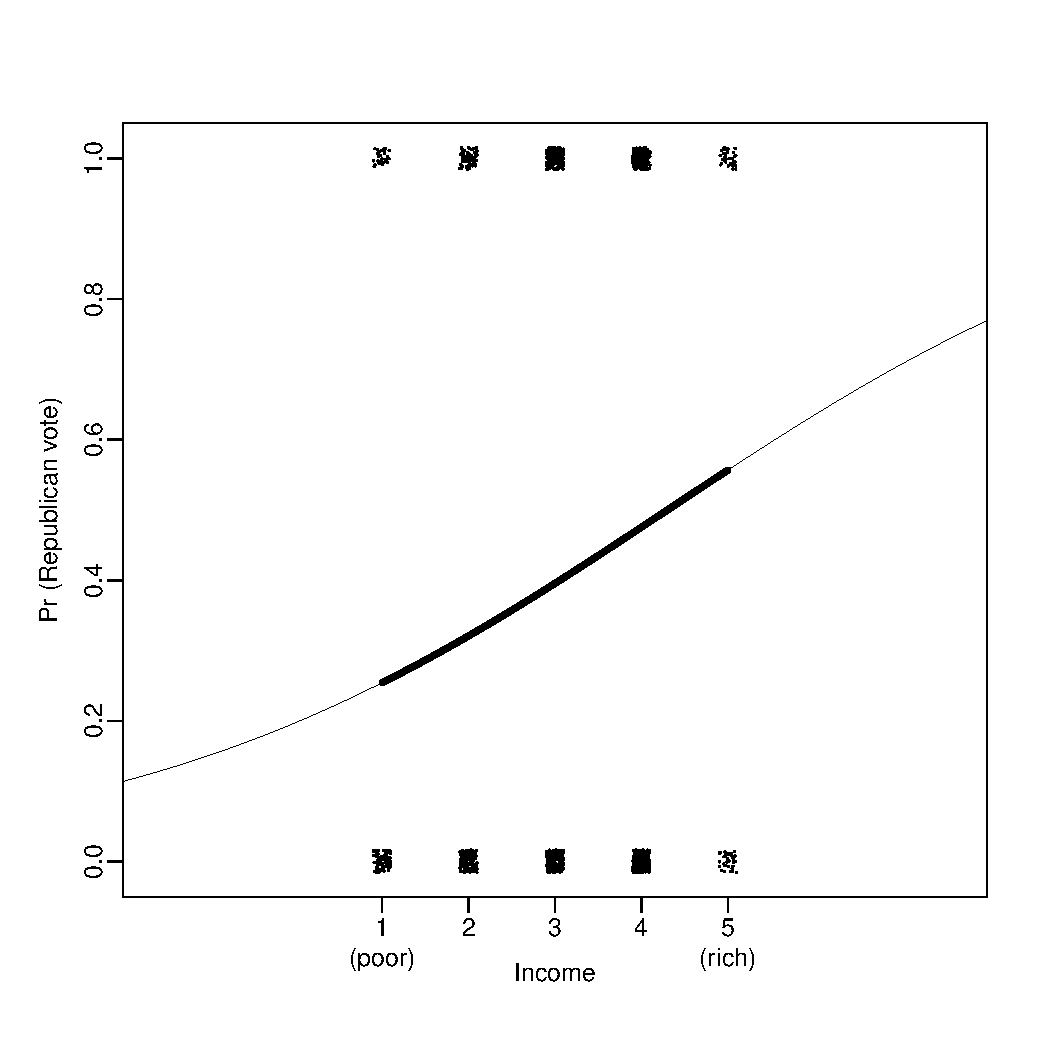
\includegraphics[width=6cm]{fitted_model.pdf}
      \caption{\textsl{Fitted model of voting-income logistic regression}}
    \end{figure}

}


\frame[t] {
  \frametitle{Interpretation of the Coefficients: Odds Ratio}
  \begin{itemize}
  \item If two outcomes have the probabilites $(p,1-p)$, then $p/(1-p)$ is called the {\color{red} odds}.
  \vskip 12pt
  \item The ratio of two odds $\frac{p_1(1-p_2)}{(1-p_1)p_2}$ is called {\color{red} odds ratio}.
  \vskip 12pt
  \item In the voting and income example, the slope of income is actually the odds ratio when income increases by {\color{red}one} category.
  \[\beta_{\text{income}}=\log\left(\frac{P(y=1)|\text{income}=k+1)}{P(y=0|\text{income}=k+1)}\Biggr/\frac{P(y=1)|\text{income}=k}{P(y=0|\text{income}=k)}\right)\]
  \vskip 12pt
  \item Folks at biostat really like odds ratio. But for some applications, odds ratio seems obscure and difficult to understand.
  \end{itemize}

}


\frame[t] {
  \frametitle{Interpretation of the Coefficients: Probability Scale}
  We take a look at the standard logistic function curve. 
    \begin{figure}[hbtp]
      \centering
      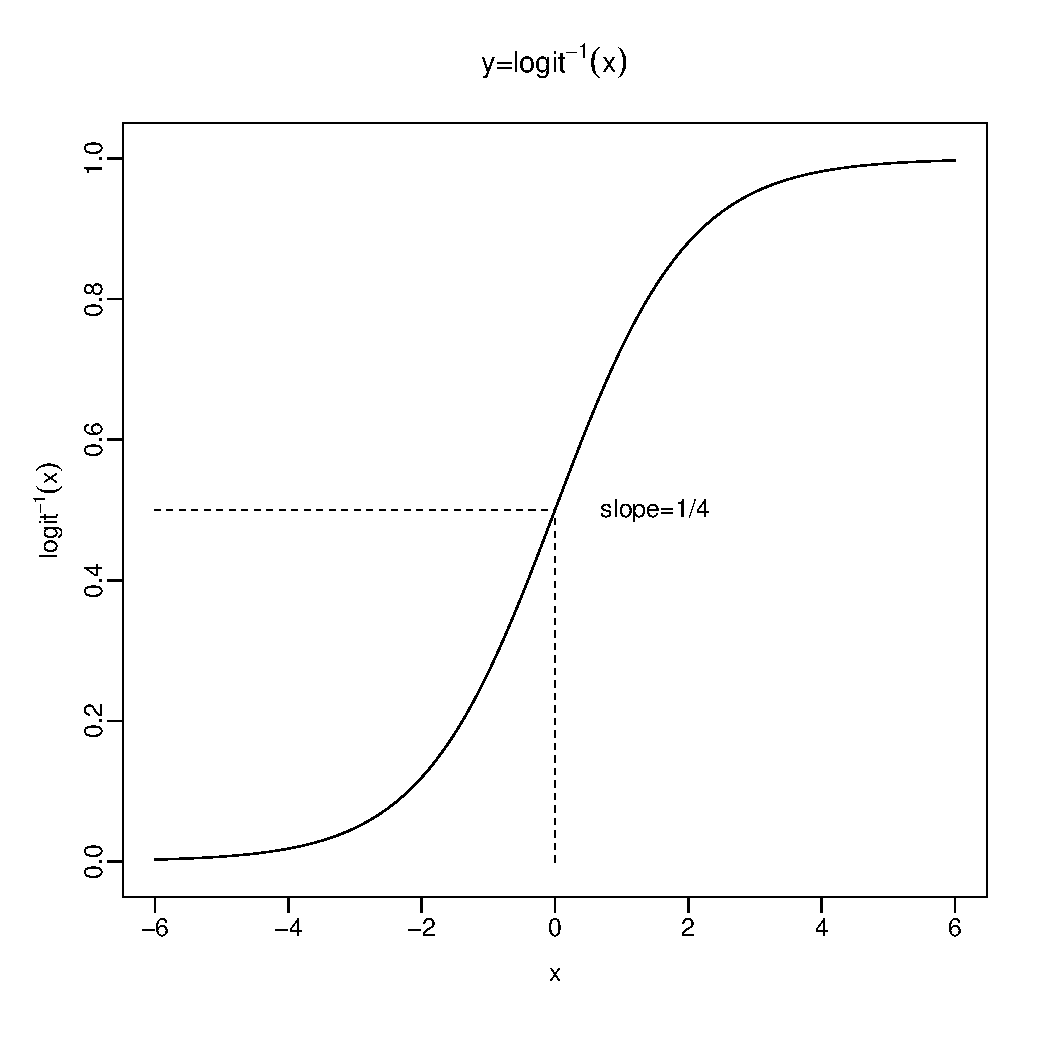
\includegraphics[width=6cm]{logistic_curve.pdf}
      \caption{Curve of inverse logistic function.}
    \end{figure}
  

}


\frame[t] {
  \frametitle{Interpretation of the Coefficients: Probability Scale}
  \begin{itemize}
  
  \item The logistic curve is steepest at its center, with slope $\beta/4$. As a rule of convenience, we can take $\beta/4$ as an upper bound of predictive difference corresponding to one unit difference in predictor. This is valid near the midpoint of the logistic curve. 
  \vskip 24pt
  \item
  In the voting-income example, the fitted model suggests that a difference of 1 in income category corresponds to at most an $.33/4\approx 8\%$ positive difference in the probability of supporting Bush.

  \end{itemize}

}


\frame[t] {
  \frametitle{Probit Model and Latent Variable Formulation}
  \begin{itemize}
  \item Another popular model for binary response data is Probit Model.
  \vskip 24pt
  \item In Probit Model, we choose a different mapping from $\mathbb{R}$ to $[0,1]$ unit interval: the CDF of standard normal. 
  \vskip 24pt
  \item If $\xi$ is a standard normal random variable and $\Phi$ is its CDF, \[p=\text{probit}(x^T\beta)=P(\xi+x^T\beta>0)=\Phi(-x^T\beta)\]

  \end{itemize}

}


\frame[t] {
  \frametitle{Probit Model and Latent Variable Formulation}
  \begin{itemize}
  \item We can view probit model in a {\color{red}Latent Variable Formulation}. Each dicrete outcome $y_i$ is associated with a continuous, unobserved $z_i$ 
  \begin{eqnarray*}
  y_i &=& \begin{cases} 1 & \text{if } z_i>0\\ 0 & \text{if } z_i<0 \end{cases}\\
  z_i &=& x_i^T\beta+\xi_i
  \end{eqnarray*}
  $\xi_i$ are i.i.d. standard normal random variables.
  \item 
  In fact, we can incorporate logistic regression model into this formulation if we let $\xi_i$ follows {\color{red}logistic distribution}, which is defined by 
  \[P(\xi_i<x)=\text{logit}^{-1}(x)\]
  \end{itemize}

}


\frame[t] {
  \frametitle{Probit Model and Latent Variable Formulation}
  \begin{itemize}
  \item A lot of statistical problems are easier to understand and tackle from a Latent Variable Formulation point of view.
  \vskip 24pt
  \item In practice, logistic regression and probit regression are not very different. In fact, logistic distribution is very close to normal distribution with mean 0 and standard deviation 1.6.
  \vskip 24pt
  \item
  So to use logistic or probit regression is mostly just a matter of taste.
  \end{itemize}

}

\frame[t]{
  \frametitle{Estimation}
  \begin{itemize}
  \item
  Unlike simple linear regression, no explicit maximum likelihood estimators can be given for logistic regression.
  \vskip 24pt
  \item
  {\color{red}Iterative Weighted Least Squares} scheme is used to estimate the parameters. In some literature, it is also called {\color{red}Fisher's Scoring Method}.
  \vskip 24pt
  \item
  We don't delve into details here.
  \end{itemize}
}

\frame[t]{
  \frametitle{Model Checking: Residuals}
  \begin{itemize}
  \item Based on the same rational of diagnostics of simple linear model, we may want to look at the {\color{red} Fitted values v.s. Residuals} plot.
  \item Because of the discreteness of the response, the plot doesn't show us much useful information.
    \begin{figure}[hbtp]
      \centering
      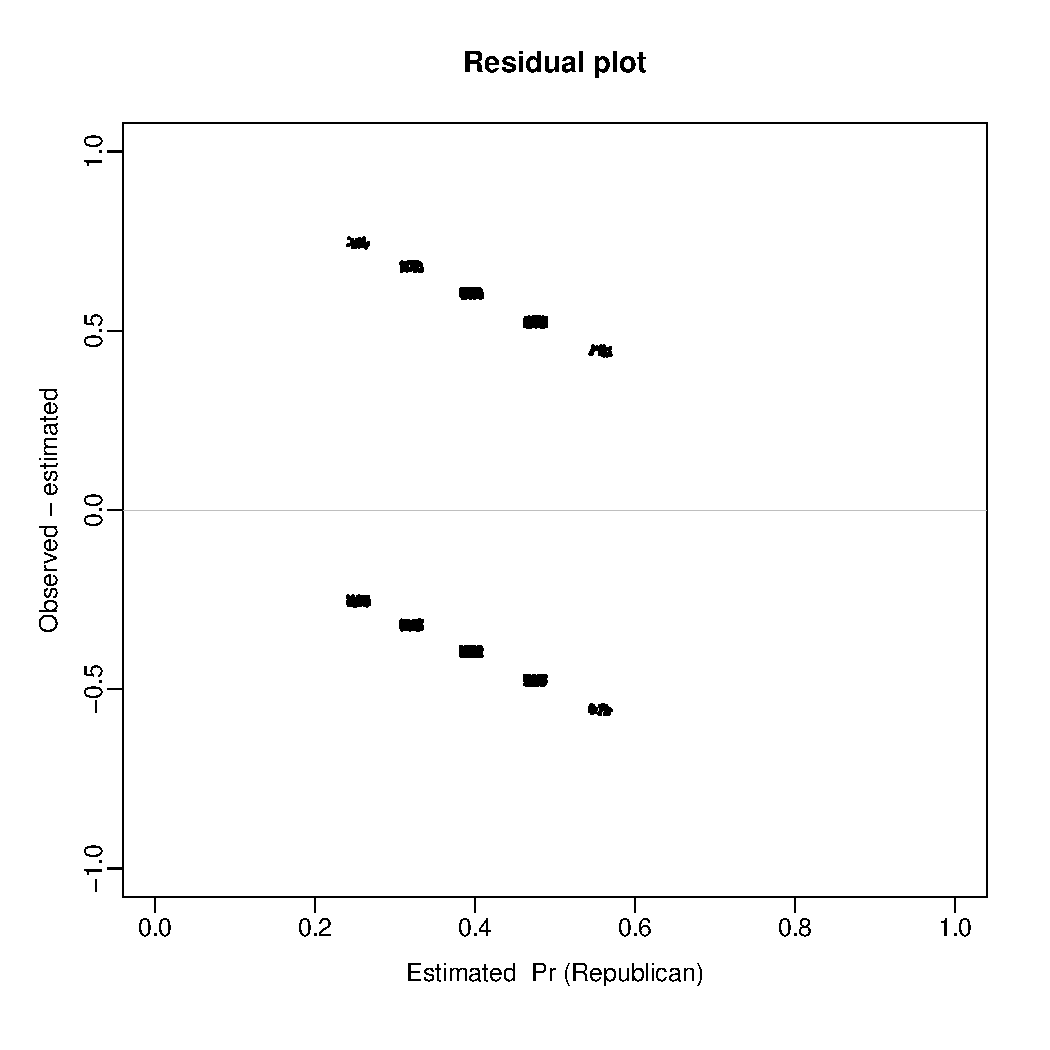
\includegraphics[width=5cm]{residual.pdf}
      \caption{Residual plot for voting-income example}
    \end{figure}
  \end{itemize}

}

\frame[t]{
  \frametitle{Model Checking: Residuals}
  \begin{itemize}
  \item
    Instead, we can look at the binned residual plot. 
    
    \begin{figure}[hbtp]
      \centering
      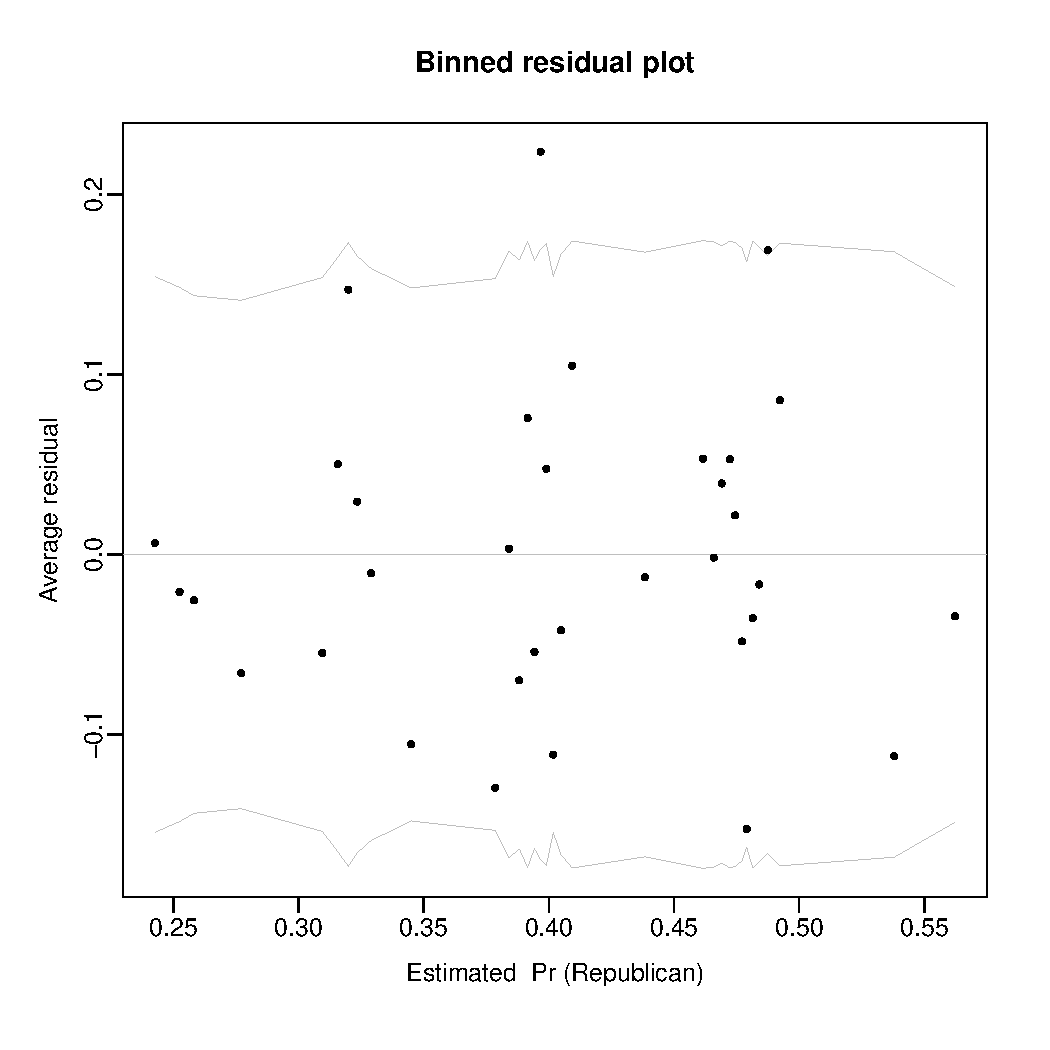
\includegraphics[width=4.5cm]{binned_residual.pdf}
      \caption{Binned residual plot for voting-income example}
    \end{figure}

  \item
  We can see that most of the points lie inside the $95\%$ interval and no dramatic pattern appears.

  \end{itemize}
}


\frame[t]{
  \frametitle{Model Checking: Error Rate}
  \begin{itemize}
  \item Another thing that we might want to look at is Error Rate.
  \vskip 24pt
  \item If we do deterministic prediction, i.e. guessing $y_i=1$ when fitted value $\text{logit}^{-1}(x_i^T\hat\beta)>.5$ and $y_i=0$ if otherwise, then we define the proportion of wrong prediciton as {\color{red} Error Rate}.
  \vskip 24pt
  \item Error Rate need to be at least less than .5(the error rate when we just randomly guess). 
  \end{itemize}
}


\frame[t]{
  \frametitle{Model Checking: Deviance}
  \begin{itemize}
  \item {\color{red}Deviance} is defined as -2 times the logarithm of the likelihood function. The better the model fit, the lower the deviance is.
  \vskip 24pt
  \item If a predictor that is random noise is added to the model, we expect deviance to decrease on average by 1.
  \vskip 24pt
  \item If a predictor that is informative is added to the model, we expect deviance to decrease on average by more than 1. The larger the increase, the more relevant the predictor is for our model.
  \vskip 24pt
  \item Deviance is a fundmental concept in model comparison and selection.
  \end{itemize}
}

\frame[t]{
  \frametitle{Model Checking: Deviance}
  \begin{itemize}
  \item For the voting-income example, the null model (only has intercept) has a deviance of 1591.
  \vskip 24pt
  \item Added income as a predictor, the model has a deviance of 1557.
  \vskip 24pt
  \item This shows that income is informative for predicting vote outcome.
  \end{itemize}
}

\frame[t]{
  \frametitle{Software Implementations}
  \begin{itemize}
  \item R: \texttt{glm}
  \vskip 24pt
  \item Matlab: \texttt{glmfit}
  \end{itemize}
}


\end{document}
